\author {Перминова Виктория}
\title{Расчётная работа}

\documentclass[a4paper,14p]{article} 

\usepackage[T2A]{fontenc}
\usepackage[russian]{babel}
\usepackage{graphicx}
\usepackage{wrapfig}
\usepackage{multicol}
\usepackage{mathtools}
\usepackage[top=2cm, bottom=2cm, left=2cm, right=2cm, footskip=15mm]{geometry}


\begin{document}
\begin{center}
  Отчёт по расчётной работе  
\end{center}

Цель работы - изучить основы теории графов, способы представления графов, базовые алгоритмы для работы с разными видами графов.

\textbf{\textit{Задание:}} реализовать код на языке `С++`, который, используя в качестве способа выражения графа матрицу инцидентности, будет находить минимальный простой разрез графа.

\textbf{\textit{Ключевые понятия:}}

\textit{Граф} - математическая абстракция реальной системы любой природы, объекты которой обладают парными связями.

\textit{Матрица инцидентности} - одна из форм представления графа, в которой указываются связи между инцидентными элементами графа (ребро(дуга) и вершина). Столбцы матрицы соответствуют ребрам, строки — вершинам. Ненулевое значение в ячейке матрицы указывает связь между вершиной и ребром (их инцидентность).

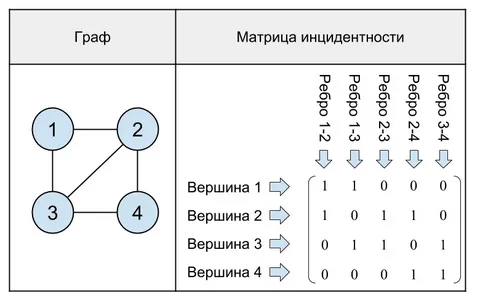
\includegraphics[width=0.8\textwidth]{матрица_инцидентности.png}

\textbf{\textit{Разрез графа}} — это разбиение вершин графа на два непустых непересекающихся подмножества.

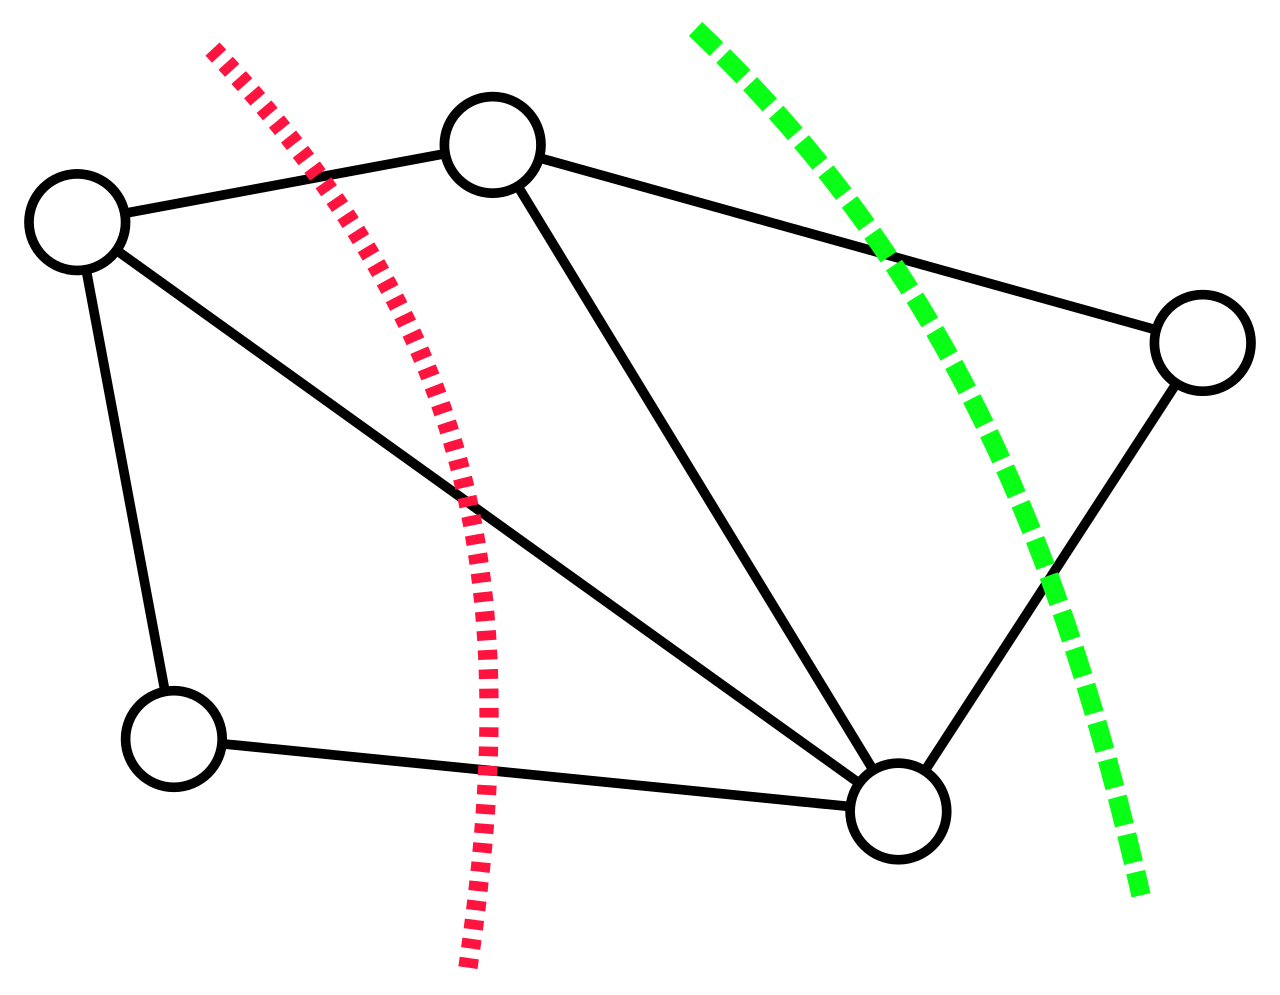
\includegraphics[width=0.8\textwidth]{разрез.png}

\textbf{\textit{Минимальный разрез графа}} — разрез, при котором размер или вес разреза не превышает размер любого другого разреза. Для невзвешенного графика минимальным разрезом будет просто разрез с наименьшим количеством ребер. Для взвешенного графика сумма весов всех ребер на разрезе определяет, является ли это минимальным разрезом.

\vspace{10pt}
\begin{center}
    \large Алгоритм выполнения задания
\end{center}
\begin{enumerate}
    \item Находим 2 строки, суммы модулей чисел в которых максимальны.
    \item Проверяем есть ли в этих строках на одинаковых местах равные элементы.
    \begin{enumerate}
        \item Если такие элементы есть, удалить столбцы с номерами этих элементов. 
        \item Если нет - вместо второй строки взять следующую по сумме модулей элементов и вернуться ко 2 пункту алгоритма.
    \end{enumerate}
    \item Прибавить вторую строку к первой.
    \item Удалить вторую строку.
    \item Пока количество строк больше 2 повторять 1-5 пункты алгоритма.
    \item Найти сумму модулей чисел первой строки в получившейся матрице.
    \item Вывести эту сумму на экран.
\end{enumerate}

\vspace{10pt}
\begin{center}
    \large Пример выполнения алгоритма
\end{center}

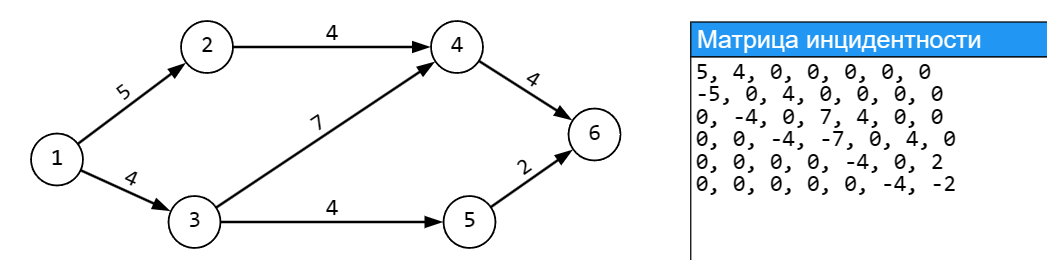
\includegraphics[width=0.8\textwidth]{пр1.png}

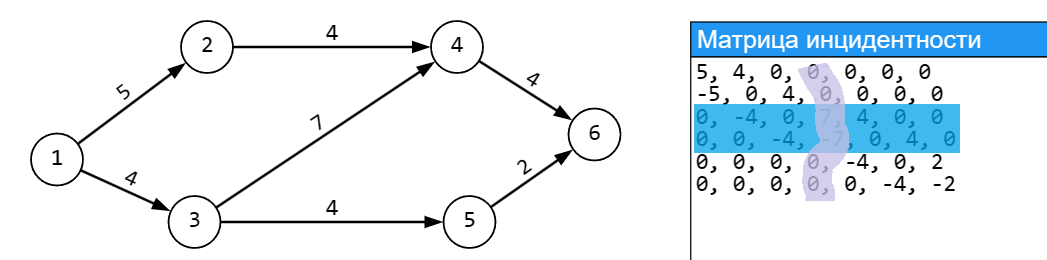
\includegraphics[width=0.8\textwidth]{пр1.1.png}

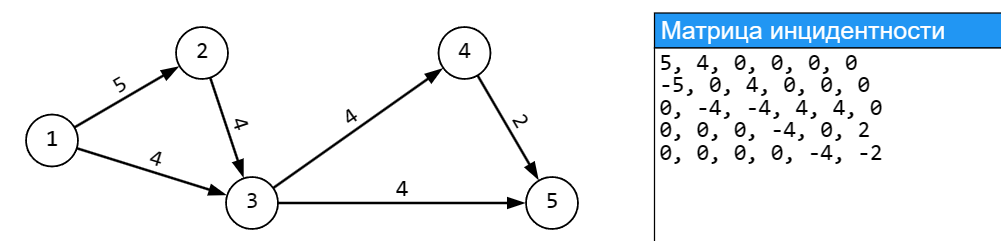
\includegraphics[width=0.8\textwidth]{пр2.png}

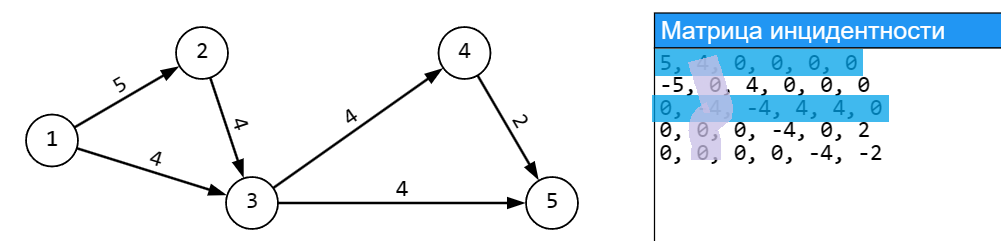
\includegraphics[width=0.8\textwidth]{пр2.1.png}

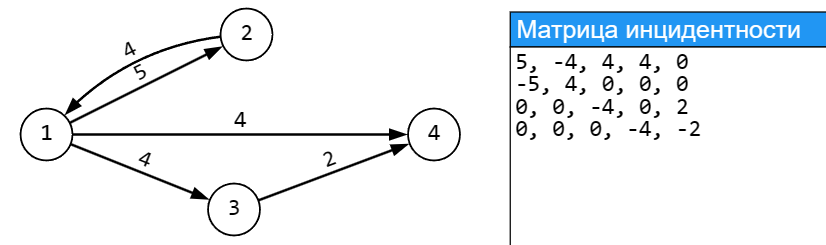
\includegraphics[width=0.8\textwidth]{пр3.png}

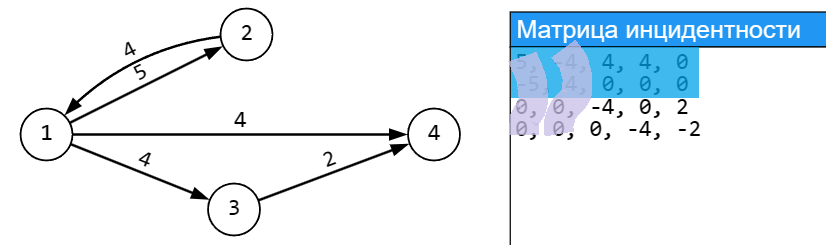
\includegraphics[width=0.8\textwidth]{пр3.1.png}

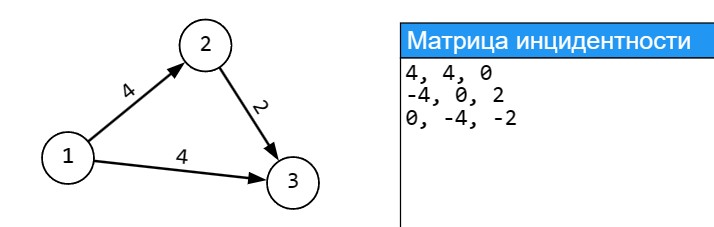
\includegraphics[width=0.8\textwidth]{пр4.png}

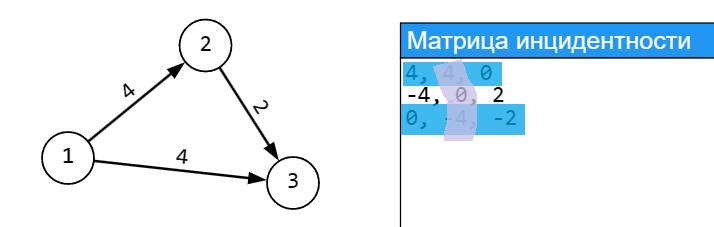
\includegraphics[width=0.8\textwidth]{пр4.1.png}

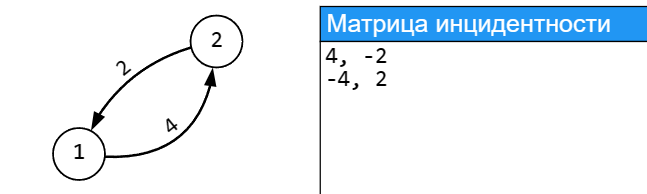
\includegraphics[width=0.8\textwidth]{пр5.png}

\vspace{10pt}
\begin{center}
    \large Код программы
\end{center}

\begin{verbatim}
#include <iostream>
#include <vector>
#include <cmath>
using namespace std;

// Функция, которая возвращает сумму модулей элементов вектора
int sum_abs(vector<int> v) {
    int sum = 0;
    for (int i = 0; i < v.size(); i++) {
        sum += abs(v[i]);
    }
    return sum;
}

// Функция, которая возвращает индекс вектора с максимальной суммой модулей элементов из списка 
векторов
int max_sum_abs_index(vector<vector<int>> v) {
    int max_index = 0;
    int max_sum = sum_abs(v[0]);
    for (int i = 1; i < v.size(); i++) {
        int curr_sum = sum_abs(v[i]);
        if (curr_sum > max_sum) {
            max_sum = curr_sum;
            max_index = i;
        }
    }
    return max_index;
}

// Функция, которая удаляет столбец с заданным индексом из матрицы
void delete_column(vector<vector<int>>& v, int index) {
    for (int i = 0; i < v.size(); i++) {
        v[i].erase(v[i].begin() + index);
    }
}

// Функция, которая прибавляет второй вектор к первому поэлементно
void add_vectors(vector<int>& v1, vector<int>& v2) {
    for (int i = 0; i < v1.size(); i++) {
        v1[i] += v2[i];
    }
}

// Функция, которая выполняет алгоритм из задания
int algorithm(vector<vector<int>> v) {
    // Пока количество строк больше 2
    while (v.size() > 2) {
        // Находим 2 строки, суммы модулей чисел в которых максимальны
        int i1 = max_sum_abs_index(v);
        vector<int> v1 = v[i1];
        v.erase(v.begin() + i1);
        int i2 = max_sum_abs_index(v);
        vector<int> v2 = v[i2];
        v.erase(v.begin() + i2);

        // Проверяем есть ли в этих строках на одинаковых местах равные числа
        bool equal_found = false;
        do {
            equal_found = false;
            for (int i = 0; i < v1.size(); i++) {
                if (abs(v1[i]) == abs(v2[i])) {
                    // Если такие числа есть, удалить столбец с номером этого места
                    delete_column(v, i);
                    v1.erase(v1.begin() + i);
                    equal_found = true;
                    break;
                }
            }
            // Если нет - вместо второй строки взять следующую по сумме модулей элементов
            if (!equal_found) {
                i2 = max_sum_abs_index(v);
                v2 = v[i2];
                v.erase(v.begin() + i2);
            }
        } while (!equal_found);

        // Прибавить вторую строку к первой
        add_vectors(v1, v2);

        // Удалить вторую строку
        v2.clear();
    }

    // Найти сумму модулей чисел первой строки в получившейся матрице
    int result = sum_abs(v[0]);

    // Вернуть эту сумму
    return result;
}

int main() {
    setlocale(LC_ALL, "Russian");
    int n, m;
    cout << "Введите количество вершин в графе: ";
    cin >> n;
    cout << "Введите количество рёбер в графе: "; 
    cin >> m;
    vector<vector<int>> v(n, vector<int>(m));
    cout << "Введите матрицу инцидентности: " << endl;
    for (int i = 0; i < n; i++) {
        for (int j = 0; j < m; j++) {
            cin >> v[i][j];
        }
    }
    int result = algorithm(v);
    cout << "Размер минимального разреза данного графа равен: " << result;
    return 0;
}
\end{verbatim}

\vspace{10pt}
\begin{center}
    \large Тестирование
\end{center}

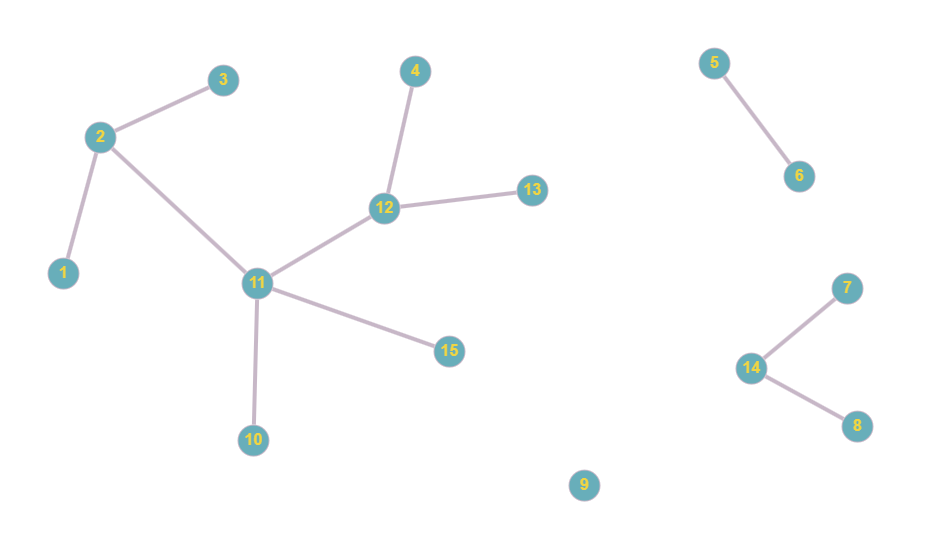
\includegraphics[width=0.45\textwidth]{graph1.png}
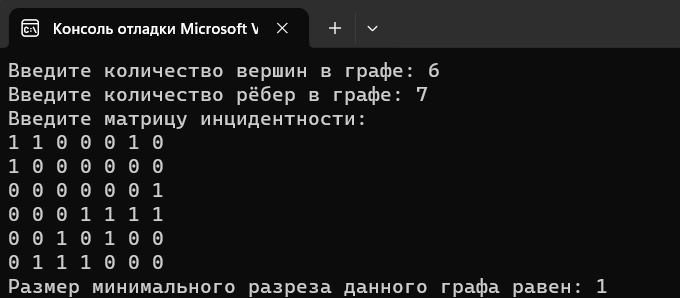
\includegraphics[width=0.45\textwidth]{mi1.png}

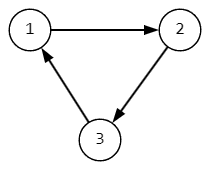
\includegraphics[width=0.45\textwidth]{graph2.png}
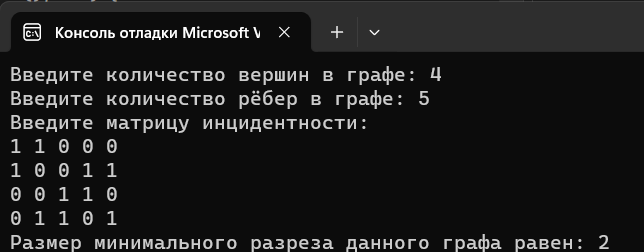
\includegraphics[width=0.45\textwidth]{mi2.png}

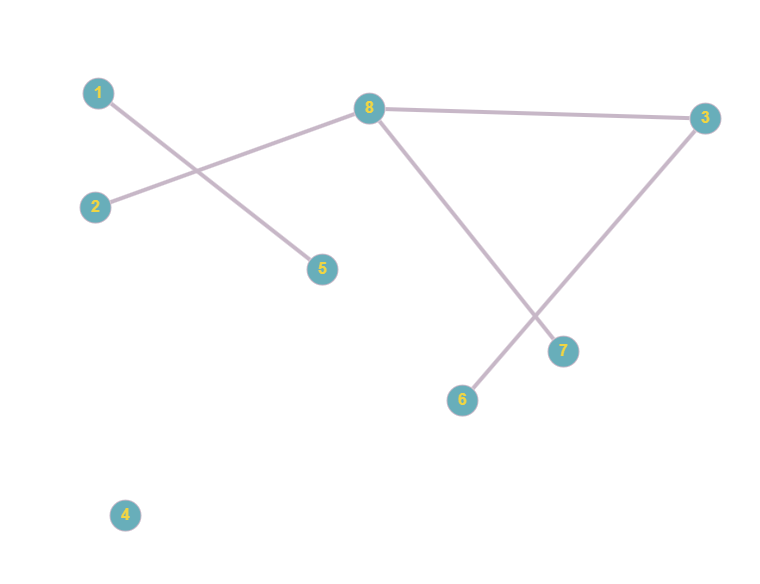
\includegraphics[width=0.45\textwidth]{graph3.png}
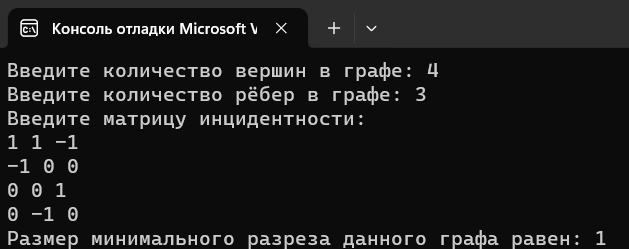
\includegraphics[width=0.45\textwidth]{mi3.png}

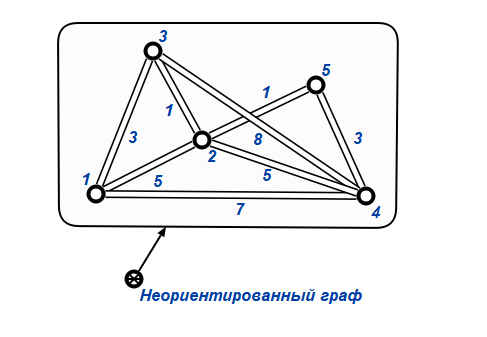
\includegraphics[width=0.45\textwidth]{graph4.png}
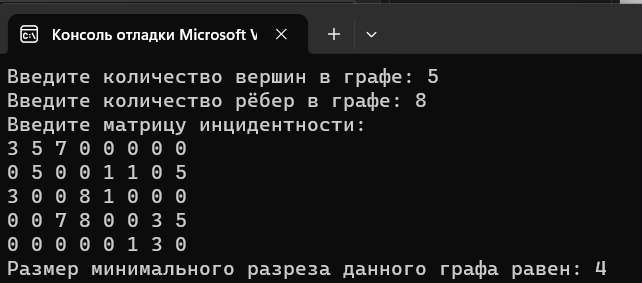
\includegraphics[width=0.45\textwidth]{mi4.png}

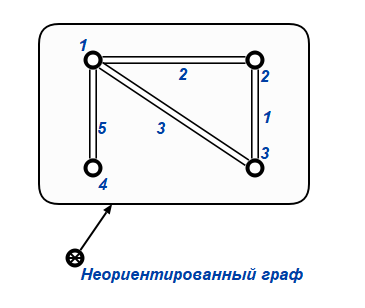
\includegraphics[width=0.45\textwidth]{graph5.png}
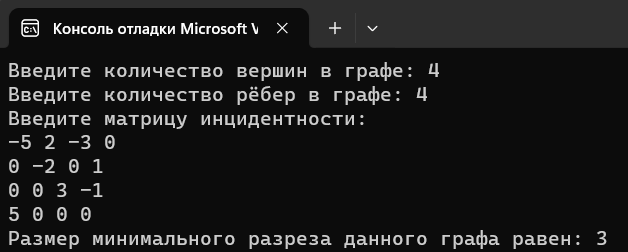
\includegraphics[width=0.45\textwidth]{mi5.png}

\vspace{10pt}
\begin{center}
    \large Выводы
\end{center}

В результате выполнения данной работы были получены следующие практические навыки:
\begin{itemize}
    \item изучены основы теории графов;
    \item изучены способы представления графов;
    \item изучены базовые алгоритмы для работы с графами.
\end{itemize}
\end{document}